% ************************************************
\chapter{Design}
\label{chp:design} % \minitoc\mtcskip % %
% ************************************************

\section{Overview}
In general, a language model is created by choosing a modeling
criterium and applying it to a a large set of observations. These
observations may be raw word sequences or annotated word sequences,
depending on the chosen criterium. Each observation is coupled with an
adjustment of the language model to maximise the score for that
particular observation type. The larger the set, the better, as each
observation makes the model a better reflection of linguistic reality.

We choose a two-phase training method and exclusively follow the
natural language processing architecture based on deep neural
networks\footnote{Details on this type of network may be found in
\vref{sec:deeplearning}.} described in \cite{collobert-2011}; all
theories and techniques described are their work and ideas, except for
the specific adaptations made to accommodate the system to ancient
Greek. We give a summary overview of the architecture as described in
the paper; subsequent sections provide more detail and specific
modifications necessary to process ancient Greek.

The first phase uses a large unlabelled corpus to create a simple
probabilistic model using a little linguistic knowledge as possible:
the goal is to assign scores to word sequences that are proportional
to the probability of these sequences being `correct', i. e. likely to
appear in real linguistic data. Maximising these scores is achieved by
corrupting data from the observation corpus; the model is then
adjusted to give the real observation a higher score than the
corrupted observation.

This method creates a structured internal representation for each word
in vector form, which define how the word is embedded within an
$n$-dimensional vector space; hence, these vectors are termed
\textbf{embeddings}. (\textit{Ne sit confusio}: note that the
components of this feature vector do not necessarily show a one-on-one
correspondence with linguistic features.)

The second phase is implemented on top of the first. The embeddings
created in the first phase are used to initialise new networks for
each of the tasks we want to train. We then use a new observation
corpus, this time equipped with annotation. We convert these
annotations to a vector form, with each vector component representing
a linguistic feature. The parameters of the network are then further
adjusted to fit the behavior of the observation corpus. The scores
returned by the model are now in vector form, each component being a
score similar to the one developed in the first phase.

Performance improvements are expected due to the fact that at this
stage, most of the general learning is actually already done and we
are applying classification to certain clusters in the vector space,
which allows the model to make more accurate inferences when
classifying rare words or phrases.

The model can then be used to generate annotation for unlabelled
sentences. Given a sequence centered around a word, a vector
containing scores for each possible tag for this central word is
returned. Prediction is handled by concatenating this type of output
for entire sentences and applying the Viterbi algorithm [described
formally in \ref{sec:viterbi}] to the resulting matrix.

\section{Network structure}
\label{sec:networkstructure}

Deep networks contain multiple layers which are sequentially trained;
the input of a layer is weighted and passed on to the following layer,
which may be either an output layer or a hidden layer. Several layers
are stacked in this manner.

\subsection{Hyperparameters}

Before constructing a network, we need to decide on a set of
hyperparameters that will influence the parameters of the neural
network and its training process. These are:

\begin{itemize}
\item the \textbf{embedding dimensions}, written $d_{wrd}$: the number
of components in a word feature vector;
\item the \textbf{dictionary size}, written $D$: how many words we
want to consider when training;
\item the \textbf{window size}, written $wsz$: the number of words we
want to consider per example;
\item the \textbf{learning rate}, written $\lambda$: when using
gradient descent, how much we want to adjust the network parameters at
each gradient step;
\item the \textbf{embedding learning rate}, written $\lambda_{e}$: the
same as $\lambda$, but for the purpose of learning embeddings -
usually smaller to limit the influence of individual observations on
the training process;
\item the \textbf{input, output and hidden size}, written $n^l_{in}$,
$n^l_{out}$, and $n^l_{hu}$, respectively: the number of neurons
contained in a layer $l$.
\end{itemize}

\begin{figure}
  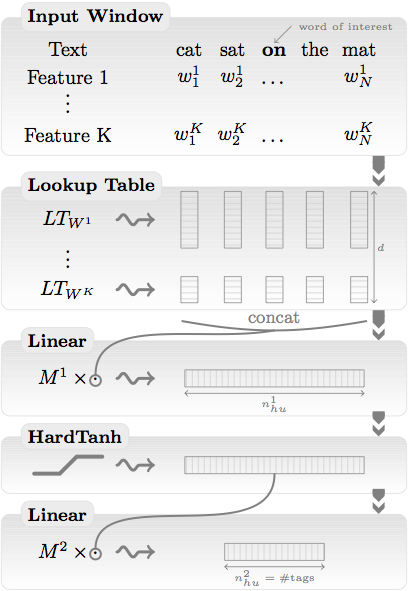
\includegraphics[width=\textwidth]{nnstructure}
  \caption{The basic network structure, using a window
approach. Figure from
\cite[2499]{collobert-2011}.} \label{fig:nnstructure}
\end{figure}

\subsection{Lookup table layer} The lookup table itself is a matrix
with $d_{wrd}$ rows and $D$ columns. Its initial construction is as
follows: given a frequency table, the $D$ most common words are chosen
and placed in order. Each word is now assigned an index according to
its ranking in the frequency table. The most common word gets index 1,
the second most common index 2 etc., up to the word in the $D^{th}$
place in the table, which is assigned index $D$. For each index, a new
embedding of size $d_{wrd}$ with small random values is created and
assigned to that index. The lookup table matrix itself is constructed
by concatenating these $D$ vectors as columns.  In this way, a lookup
operation for an index $i$ is actually nothing more than the selection
of the $i^{th}$ column from this matrix.

The lookup table layer itself consists of $wsz$ input neurons; given a
text window, each word is converted to its corresponding index, which
is then fed to the neuron corresponding to its position in the window,
which retrieves the embedding of that word from the lookup table. The
output of all neurons is then concatenated into a single matrix, whose
columns are now the embeddings for the input window.

Formally, given a word index vector $w \in N^{wsz}$ and a lookup table
$L \in R^{d_{wrd} \times D}$, we can express this as as a function
$LT$:

\begin{equation} \label{eq:ltmatrix} LT(L, w) =
\left( \begin{array}{cccc} L_{1,w_1} & L_{1,w_2} & \ldots &
L_{1,w_{wsz}} \\ L_{2,w_1} & L_{2,w_2} & \ldots & L_{2,w_{wsz}} \\
\ldots & \ldots & \ldots & \ldots \\ L_{d_{wrd},w_1} & L_{d_{wrd},w_2}
& \ldots & L_{d_{wrd},w_{wsz}} \end{array} \right)
\end{equation}

An interesting feature of this type of representation is that it is in
fact a highly performant abstraction for the classic $n$-gram. In most
NLP architectures $n$ is given a relatively low value in order to
limit computational expenses; the Google $n$-gram project, which is the
largest of its kind, limits itself to five-grams. N-grams are also
used differently: the first $n - 1$ words serve as the context for the
$n^{th}$ word in the $n$-gram. Here, we can take advantage of the
purely numerical form of text window embeddings by choosing a somewhat
larger text window size and considering the central column in such
windows in its full context, both prior and posterior.

\subsection{Linear layer}
A linear layer takes a fixed size vector and performs a linear
operation on it: the dot product of this vector with a set of
parameters $W$ is computed and a bias added. Formally, given the
output vector $f^{l-1}_\theta$ of layer $l-1$, the following
computation is performed in layer $l$:
\begin{equation}
  f^l_\theta = W^l \cdot f^{l-1}_\theta + b^l
\end{equation}
Where $\theta$ indicates the existing parameters of the network and
$W^l \in R^{n^l_{hu} \times n^{l-1}_{hu}} $ and $b^l \in R^{n^l_{hu}} $
are the parameters of the layer to be trained, with $n^l_{hu}$
representing the amount of hidden units in layer $l$. Linear layers
transform their input and several such layers can be stacked, similar
to how linear functions can be composed.

\subsection{Hard hyperbolic tangent layer}

If we intend for our network to be able to model a highly nonlinear
system such as language, we need to introduce nonlinearity
somewhere. A good function for this is the hyperbolic tangent, which
is differentiable everywhere and approximates a linear threshold
function very nicely. A layer $l$ using the hyperbolic tangent as an
activation function contains $n^l_{hu}$ neurons taking $n^{l-1}_{hu}$
inputs. In this case, the activation function $g(x)$ for a scalar x
is:
\begin{equation}
  g(x) = tanh(x) = \frac{e^{2x} - 1}{e^{2x} + 1}
\end{equation}
For an input vector generated by a layer $l - 1$, the function $g$ represented by a hyperbolic tangent layer can be defined as:
\begin{equation}
  f^l_{\theta} = g(f^{l-1}_{\theta})
  = \left[ \begin{array}{c}
      g(f^l_{\theta1}) \\
      g(f^l_{\theta2}) \\
      \ldots \\
      g(f^l_{\theta n^{l-1}_{hu}})\\ \end{array} \right]
\end{equation}
We approximate this function using the hard hyperbolic tangent, defined for a scalar as:
\begin{equation}
  hardtanh(x) = = \begin{cases} 1, & \mbox{if } x > 1 \\ -1, & \mbox{if } x < -1 \\ x & \mbox{otherwise.}\end{cases}
\end{equation}
We can define this function for vector inputs in the same manner
as for the hyperbolic tangent function.

\subsection{Scoring layer}

The final layer. This is actually simply a linear layer which is
designed to output a vector containing as many elements as there are
possible tags for the task at hand. Each output element is a score
which reflects the probability of the corresponding tag for the
central word in the input window.

\section{Phases of learning}
\subsection{Unsupervised learning}
\label{sec:unsupervised}

The first phase of learning is unsupervised; large amounts of raw
language data are fed to the network. Instead of training using a
classical squared-loss function, a pairwise ranking function is
introduced. The network is constructed as described in the previous
section; we want a single score $f_{\theta}(x)$ to be output for a
given window of text $x$.  The window is first corrupted using a word
$w$ from the dictionary by replacing the central word in $x$ by
$w$. We express this corrupted window as $x^{(w)}$. The pairwise
ranking of any two such pairs $x$ and $w$ is defined as $r(\theta, x, w) = max\left\{0,
  1 - f_{\theta}(x) + f_{\theta}(x^{(w)})\right\}$. 
In effect, we want the non-corrupted window to achieve a higher score
than the corrupted window. We can achieve this by adjusting the
parameters $\theta$ such that the pairwise ranking of $x$ and $w$ is
minimal, since this implies that $f_{\theta}(x)$ must yield a higher
score than $f_{\theta}(x^{(w)})$.

Summing this operation over all possible pairs $(x, w)$ and defining a
mapping from the parameters $\theta$ to this sum, we obtain a general
cost function:
\begin{equation}
  \theta \mapsto \sum\limits_{x \in X} \sum\limits_{w \in D} r(\theta, x, w)
\end{equation}
Where $X$ is the set of possible windows of size $wsz$ and $D$ the chosen
dictionary. Minimizing this function with respect to $\theta$ will
ensure the relevant parameters (the embeddings and the first two
layers) are tuned so that our ranking function $f_{\theta}$ yields
accurate scores. 

Using this simple criterion, we have a method for crafting a set of
parameters that contains a consistent structured internal
representation of the training data. Despite the relatively simplicity
of the criterion, the huge amounts of parameters results in a very
taxing and lengthy computation. Furthermore, there is no guarantee
that the cost function has a single minimum with respect to $\theta$;
a full grid search would be necessary, which necessitates vast amounts
of computing time.

Instead, the process is sped up using \textbf{curriculum learning};
the basic idea of this technique is analogous to the learning process
children are put through in school: instead of starting their
education with university-level quantities of difficult material
immediately, a restricted set of elementary concepts is introduced on
which they concentrate. Successive phases of learning are performed by
gradually expanding the set of concepts which is to be learned, making
use of earlier concepts to facilitate the understanding of more
complex concepts.

The same method, for reasons not yet fully understood, can be applied
to unsupervised learning.\footnote{Among the scholarship of note on
  this subject we find \citet{bengio2009curriculum} and
  \citet{erhan2010}.} First, the training material is restricted to the
most frequent observations of the process we want to model. Training
over this restricted set creates a simplified model which, due to the
abundance of examples, should be accurate. Subsequently, new
iterations of the learning algorithm are run over successively larger
sets; at each iteration, the model becomes more detailed and describes
more classes of observations more accurately.

This is applied to the problem at hand by choosing
successively larger dictionary sizes. During the calculation of the
minimum of the cost function, windows which are not centered around a
word which is in the dictionary are ignored. This initially entails a
significant reduction of our sets $X$ and $D$, which makes the process
a bit less computationally demanding. Subsequent iterations are
computationally more expensive, but are initialised with the
parameters found by previous iterations; observations previously used
in learning will already return excellent scores and will only
necessitate minor adjustments to the parameters, while new
observations can be fit into the general picture more easily.

We note that we do not generate all possible corrupt windows for
parameter adjustment each time we treat a text window. Instead, at
each window, we pick a random word with which to corrupt the window;
we improve the model by running the learning algorithm for several
epoch; this type of training minimises the time to process a training
corpus once but can be run indefinitely. We can set a number of epochs
to run successively, and define a validation criterium for
transitioning to the next epoch.

\subsection{Supervised learning}
\label{sec:supervised}

The supervised training phase involves the creation of task-specific
networks which are initialised with the embeddings created during the
unsupervised phase; these form a shared first part of all networks. A
given network is then tailored to have an adapted output as necessary
for the task of interest. Training proceeds in the classical fashion,
by providing correctly formatted examples and adjusting all parameters
(including the shared ones) to minimize the squared error.

The output of a network of this type is a vector; each specific
feature is encoded in on component of this vector by setting this
component to one and all others to zero. This is called a one-hot
vector. All tasks are jointly trained, that is to say, the networks
share parameters, are trained simultaneously and are allowed to modify
shared parameters. Individual (non-shared) network parameters are
modified only during training for a specific task. This technique
allows us to generalise the training benefit from each example.

\section{Adapting the architecture for ancient Greek}
\label{sec:adaptation}

Composing such a one-hot vector is not simple for Greek morphology:
any given word will belong to multiple morphological categories. For
instance, a verbal form has a tense, a mood, a number, a person, and
sometimes even a case and gender. Gathering all possible features into a
single one-hot vector is therefore not feasible.

We could approach this problem in different ways. An instinctive test
is to simply feed the system raw parses and assign one component of
the output vector to each possible parse. This is needlessly
complicated; if we look at the list of morphological parses from the
Perseus database, we find more than 2000 distinct morphological
analyses! An output vector of this size is simply too unwieldy.

A more dynamic approach would be to create one-hot vectors for each of
the following categories, with the number of options assigned to each
category corresponding to the number of components in the
corresponding output vector:

\begin{itemize}
\item major part of speech: verb, noun, adjective, pronoun, particle,
  adverb, numeral, preposition, conjunction, interjection;
\item minor part of speech: article / determinative, personal,
  demonstrative, indefinite, interrogative, relative, possessive,
  reflexive, reciprocal, proper;
\item person: first, second, third;
\item number: singular, plural, dual;
\item tense: present, imperfect, aorist, perfect, pluperfect,
  future, future perfect;
\item mood: indicative, subjunctive, optative, imperative,
  infinitive, participle, gerundive, gerund, supine;
\item voice: active, middle, passive, middle-passive;
\item gender: masculine, feminine, neuter, common;
\item case: nominative, genitive, dative, accusative, ablative,
  vocative;
\item degree: comparative, superlative.
\end{itemize}

\begin{table}
  \begin{tabular}{|l|l|l|}
    \hline
    \textbf{field}            & \textbf{category} & \textbf{possible values} \\ \thickhline
    first field  & lemma type & \specialcell{a - adjective\\c - conjunction\\d - adverb\\e - exclamation\\g - particle\\l - article\\m - numerals\\n - noun\\p - pronoun\\r - preposition\\t - participle\\v - verb\\x - miscellanea} \\ \hline
    second field & person & \specialcell{1 - first person\\2 - second person\\3 - third person} \\ \hline
    third field  & number & \specialcell{d - dual\\p - plural\\s - singular} \\ \hline
    fourth field & tense & \specialcell{a - aorist\\f - future\\i - imperfect\\l - pluperfect\\p - present\\r - perfect\\t - future perfect} \\ \hline
    fifth field & mood & \specialcell{g - gerund \\ p - participle \\ i - indicative\\m - imperative\\n - infinitive\\o - optative\\s - subjunctive} \\ \hline
    sixth field & diathesis & \specialcell{a - active\\e - energetic\\m - medial\\p - passive} \\ \hline
    seventh field & gender & \specialcell{f - feminine\\m - masculine\\n - neuter\\ o, p and q - unclear} \\ \hline
    eighth field & case & \specialcell{a - accusative\\d - dative\\g - genitive\\n - nominative\\v - vocative} \\ \hline
    ninth field & degree of comparison & \specialcell{c - comparative\\s - superlative} \\ \hline
    \hline
  \end{tabular}
  \caption{The Perseus ennealiteral morphological abbreviation system.} \label{table:perseusmorph}
\end{table}

\begin{table}
  \begin{tabular}{|l|l|l|}
    \hline
    \textbf{field}            & \textbf{category} & \textbf{possible values} \\ \thickhline
    first field & person & \specialcell{1 - first person\\2 - second person\\3 - third person} \\ \hline
    second field  & number & \specialcell{d - dual\\p - plural\\s - singular} \\ \hline
    third field & tense & \specialcell{a - aorist\\f - future\\i - imperfect\\l - pluperfect\\p - present\\r - perfect\\t - future perfect} \\ \hline
    fourth field & mood & \specialcell{i - indicative\\m - imperative\\n - infinitive\\o - optative\\s - subjunctive} \\ \hline
    fifth field & diathesis & \specialcell{a - active\\e - energetic\\m - medial\\p - passive} \\ \hline
    sixth field & gender & \specialcell{f - feminine\\m - masculine\\n - neuter} \\ \hline
    seventh field & case & \specialcell{a - accusative\\d - dative\\g - genitive\\n - nominative\\v - vocative} \\ \hline
    eighth field & degree of comparison & \specialcell{c - comparative\\s - superlative} \\ \hline
    ninth field & placeholder column & \specialcell{-} \\ \hline
    tenth field & inflectibility & \specialcell{i - inflected\\n - not inflected} \\ \hline
    \hline
  \end{tabular}
  \caption{The PROIEL decaliteral morphological abbreviation system.} \label{table:proielmorph}
\end{table}

\begin{table}
  \begin{tabular}{|l|l|l|}
    \hline
    \textbf{field}            & \textbf{value} & \textbf{Perseus first field equivalent} \\ \thickhline
    A- & adjective & $\rightarrow$ a \\ \hline
    C- & paratactic conjunctions & $\rightarrow$ c \\ \hline
    Df & adverbs & $\rightarrow$ d \\
    Dq & adverbial response particles (where, how, etc.) & $\rightarrow$ g \\
    Du & adverbial question particles (where, how, etc.)  & $\rightarrow$ g \\ \hline
    F- & Hebrew loan words & $\rightarrow$ x \\ \hline
    G- & hypotactic conjunctions & $\rightarrow$ c \\ \hline
    I- & illocutive particles & $\rightarrow$ g \\ \hline
    Ma & cardinal numerals & $\rightarrow$ m \\
    Mo & ordinal numerals & $\rightarrow$ m \\ \hline
    Nb & nouns (in general) & $\rightarrow$ n \\
    Ne & nouns (proper names) & $\rightarrow$ n \\ \hline
    Pc & pronouns (reciprocative) & $\rightarrow$ p \\
    Pd & pronouns (demonstrative) & $\rightarrow$ p \\
    Pi & pronouns (interrogative) & $\rightarrow$ p \\
    Pk & pronouns (reflexive) & $\rightarrow$ p \\
    Pp & pronouns (personal) & $\rightarrow$ p \\
    Pr & pronouns (relative) & $\rightarrow$ p \\
    Ps & pronouns (possessive) & $\rightarrow$ p \\
    Px & pronouns (quantitative, i.e.\ some, all, none, same, other) & $\rightarrow$ x \\ \hline
    R- & prepositions & $\rightarrow$ r \\ \hline
    S- & article & $\rightarrow$ l \\ \hline
    V- & verb & $\rightarrow$ v \\ \hline
    \hline
  \end{tabular}
  \caption{The PROIEL biliteral lemmatic abbreviation system.} \label{table:proiellemmata}
\end{table}

\begin{table}
  \begin{tabular}{|l|l|}
    \hline
    \textbf{The Perseus system} & \textbf{The PROIEL system} \\ \thickhline
    \begin{minipage}{2.5in}
      \begin{itemize}[noitemsep,topsep=0pt,parsep=0pt,partopsep=0pt]
      \item adv: adverbial;
      \item apos: apposing element;
      \item atr: attributive;
      \item atv/atvv: complement;
      \item auxc: conjunction;
      \item auxg: bracketing punctuation;
      \item auxk: terminal punctuation;
      \item auxp: preposition;
      \item auxv: auxiliary verb;
      \item auxx: commas;
      \item auxy: sentence adverbials;
      \item auxz: emphasizing particles;
      \item coord: coordinator;
      \item exd: ellipsis;
      \item obj: object;
      \item ocomp object complement;
      \item pnom: predicate nominal;
      \item pred: predicate;
      \item sbj: subject.
      \end{itemize}
    \end{minipage} &
    \begin{minipage}{2.5in}
      \begin{itemize}[noitemsep,topsep=0pt,parsep=0pt,partopsep=0pt]
      \item adnom: adnominal;
      \item adv: adverbial;
      \item ag: agens;
      \item apos: apposition;
      \item arg: argument (object or oblique);
      \item atr: attribute;
      \item aux: auxiliary;
      \item comp: complement;
      \item expl: expletive;
      \item narg: adnominal argument;
      \item nonsub: non-subject (object, oblique or adverbial);
      \item obj: object;
      \item obl: oblique;
      \item parpred: parenthetical predication;
      \item part: partitive;
      \item per: peripheral (oblique or adverbial);
      \item pid: Predicate identity;
      \item pred: predicate;
      \item rel: apposition or attribute;
      \item sub: subject;
      \item voc: vocative;
      \item xadv: open adverbial complement;
      \item xobj: open objective complement;
      \item xsub: external subject.
      \end{itemize}
    \end{minipage} \\ \hline
  \end{tabular}
  \caption{The Perseus and PROIEL syntactic annotation systems.} \label{table:proielmorph}
\end{table}

This approach has its downside: we now have to train distinct networks
for each network. The upside, though, is that each of these networks
is much, much smaller than a single network mapping all possible
parses and will be easier to train; an example of the
divide-and-conquer technique. We could possibly be confronted with
impossible parses, such as an 'imperfect optative', but this is highly
unlikely due to the total absence of examples for this form.

The task of preprocessing the corpus, which is discussed
\textit{infra}, is also simplified due to this approach: the two main
corpora from which the training material is gathered use similar but
slightly different annotation schemes. The PROIEL system is a bit more
complex, but essentially gives the same information as the Perseus
system. Tables 1 and 2 offer a detailed overview of both systems;
table 3 contains conversion guidelines. For simplicity's sake, we pick
the Perseus system, since this limits the amount of networks we'd have
to train to nine. Instead of having to convert from one type of
annotation to another, we can simply split the annotations into their
constituent parts, store them in different files and resolve any
annotational differences afterwards with minimal headaches.

The process of dependency annotation only requires one network, but is
a bit more complex. The source corpora for the training data once
again use similar annotation schemes but with different emphases. We
enumerate the tags for the Perseus and the PROIEL annotation system,
respectively.

We see in table 4 that they respectively use nineteen and twenty-four
different features. The Perseus system is less detailed than the
PROIEL system, but by virtue of this fact also less complex. A
possible approach is to map overlaps in both systems and find the
simplest possible tag set which can be derived from that. We can
immediately make a one-hot vector from this, since all annotated words
are equipped with a single syntactic tag. 

Another approach is provided in \cite{conf/lrec/LeeH10}, who attempt
to port the Perseus treebank to the PROIEL format. The approach has
its downside: the authors try to convert every detail of the Perseus
treebank format to the PROIEL format and achieve an accuracy rate
which still necessitates human postprocessing. We will consider it
feasible to switch to their system once a full-fledged conversion from
one scheme to the other has been carried through to completion. Until
then, we apply a simpler system with reduced information
density. Since we do not have to cope with head-dependency relations,
we use the simpler approach to reduce computational overhead in our
experimental setup.
